\section{Muestra}

Para la gestión de la matriz de LEDs se ha optado por la utilización de un sistema basado en un microcontrolador, junto con diversos drivers que faciliten la programación y la adecuación de las señales. Aunque podría haberse gestionado toda la lógica desde el ordenador, esto habría vuelto el sistema directamente dependiente de éste, lo cual impediría su funcionamiento cuando estuviera apagado. La externalización de la lógica nos permite utilizar el ordenador únicamente para enviar el contenido a mostrar en la matriz, obteniendo un sistema autónomo una vez recibida la información. Si quisiéramos mostrar información preprogramada, en lugar de definir el contenido dinámicamente, el microcontrolador nos da la opción de cargar la información durante el diseño.

Asimilando las ventajas de implementar la lógica de forma externa al ordenador, el microcontrolador se muestra como una de las opciones, entre las cuales también debemos valorar el uso de FPGAs, CPLDs o VLSIs. El diseño con VLSIs y CPLDs resulta excesivamente complejo, debido a la necesidad de efectuar operaciones aritméticas de cierta complejidad y el uso de diversos registros. El diseño se complicaría lo suficiente como para no resultar rentable por el tamaño final del circuito y el número de integrados necesarios. Las FPGAs suplen a la perfección estas necesidades, pero su alimentación resulta más compleja que la de un microcontrolador, y el hecho de disponer de memoria volátil complica la implementación física, al ser necesaria la adición de elementos de memoria para evitar tener que programarlas en cada arranque. Además, ninguna de las opciones anteriores incorpora periféricos específicos para la temporización o la comunicación serie. Estos recursos deberían ser desarrollados por el diseñador. Por estas razones, un sistema microcontrolador se muestra como la mejor opción, al aunar la simplicidad de diseño del circuito y la complejidad de recursos necesaria para esta aplicación.

De entre los muchos microcontroladores disponibles en el mercado, se ha utilizado el modelo Atmega48 de Atmel\cite{atmega48}, con arquitectura AVR\cite{avr}. La elección de este modelo responde a la facilidad de acceso a los recursos para trabajar con él, pues el desarrollador ha tenido a su disposición un kit de desarrollo STK500\cite{stk500} del mismo fabricante. El modelo citado dispone de recursos suficientes para el sistema a desarrollar y permite la evolución de este de cara a añadir funcionalidades en futuras versiones. Además, la arquitectura AVR se diseñó específicamente para la ejecución eficiente de código C compilado, lenguaje utilizado por el desarrollador.

En cualquier caso, y dado que no se hace uso de recursos sólo disponibles en la arquitectura AVR, con la debida adecuación del código podría utilizarse cualquier otro microcontrolador para el cual se disponga de un compilador de C, ya sean los muy extendidos PIC\cite{pic} de Microchip, aquellos compatibles con el 8051\cite{8051} de Intel, u otros muchos disponibles en el mercado.

\subsection{Elección de componentes y esquema electrónico}

Antes de abordar la elección de componentes para el circuito, se ha efectuado una división basada en la funcionalidad de éstos\footnote{El esquema electrónico completo se encuentra en el \hyperref[anexob]{Anexo B}}. A saber:

\begin{itemize}
  \item{Circuito base: agrupa los componentes básicos para el funcionamiento del sistema basado en un microcontrolador, independientemente de su uso}
  \item{Recepción: agrupa los componentes necesarios para la recepción de la información según el estándar RS232, cuyo uso se ha justificado en la sección \ref{sec:transmision}.}
  \item{Muestra: agrupa los componentes necesarios para mostrar la información.}
\end{itemize}

\subsubsection{Circuito base}

Como resulta evidente, el componente principal necesario es el microcontrolador. De entre los muchos empaquetados disponibles\cite{atmega48}, se ha escogido el PDIP de 28 contactos. Esta elección se justifica por la facilidad de montaje. Debido a la naturaleza didáctica de este proyecto y puesto que es la primera vez que el autor utiliza muchos de los recursos, este empaquetado facilita el montaje de pequeños circuitos de prueba, el cambio de dichos circuitos al kit de desarrollo y viceversa, etc.

Para el correcto funcionamiento en esta aplicación en concreto, basta con alimentar el dispositivo con una tensión de aproximadamente 5v. Para ello, conectaremos una fuente al contacto 7 (Vcc) y la masa a los contactos 8 y 22 (GND). También deberemos conectar el contacto 20 (AVCC) a la tensión de alimentación, pues a pesar de no utilizar el conversor A/D, resulta necesario para un funcionamiento adecuado del circuito.

El modelo utilizado dispone de un oscilador RC interno que genera la señal de reloj (de hasta 8Mhz) necesaria para el funcionamiento del dispositivo. Aunque éste podría ser suficiente para muchas aplicaciones, la precisión no es todo lo buena que desearíamos para garantizar una comunicación serie fiable. Al tratarse de una comunicación asíncrona, las temporización cobra una importancia vital y por lo tanto deberemos disponer de una señal de reloj más estable.

Debido a que el microcontrolador dispone de los componentes y los contactos\cite{atmega48} (9:XTAL1 y 10:XTAL2) necesarios para amplificar y utilizarlo, y puesto que su uso está muy extendido, emplearemos un cristal oscilador externo. La frecuencia de éste, 11,0592 MHz, se ha escogido teniendo en cuenta los criterios de programación para la comunicación serie asíncrona. Pueden consultarse los detalles en la sección \ref{subsec:programacion}.

El uso de un oscilador externo de cristal exige la utilización de dos condensadores cerámicos de idéntica capacidad, tal como puede verse en la figura \ref{fig:esq_osc}. El valor de éstos, atendiendo a la información contenida en la hoja de características del microcontrolador\cite{atmega48}, se ha definido como 22pF.

\begin{figure}[!htp]
\centering
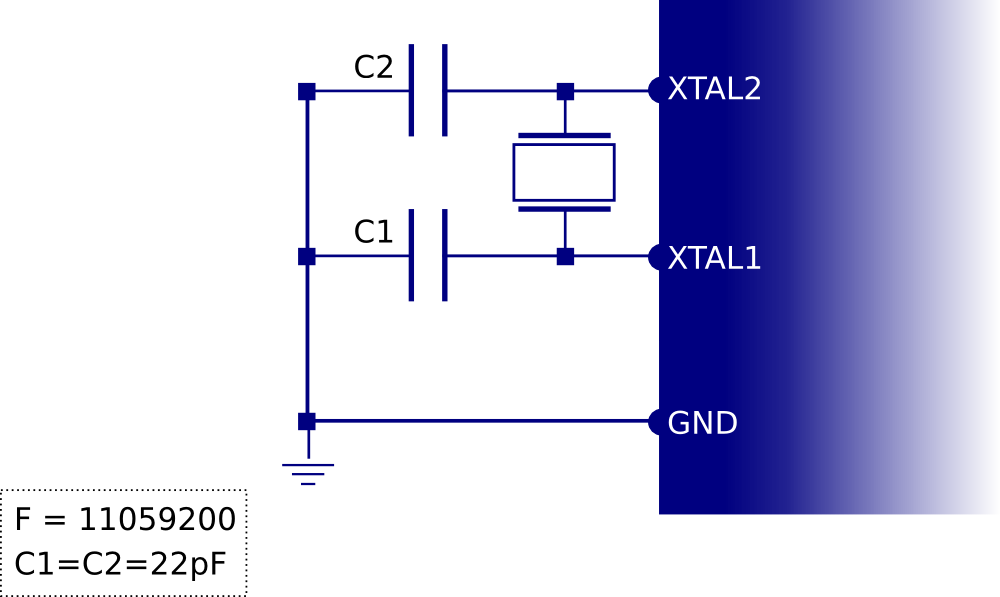
\includegraphics[width=300pt]{./images/esq_osc.png}
\caption{Esquema de conexión del oscilador externo.}
\label{fig:esq_osc}
\end{figure}

\subsubsection{Recepción}

Como el microcontrolador dispone de un periférico específico para la implementación de comunicaciones serie que permite el modo de trabajo asíncrono con dos contactos asociados en el empaquetado, siempre y cuando la señales sean TTL compatibles, no es necesaria la adición de ningún componente externo.

Tal como se ha descrito en la sección \ref{subsec:trans_fis}, las señales provenientes del ordenador se adecuan mediante el circuito integrado MAX232\cite{max232} a niveles apropiados. Simplemente se debe conectar la salida adecuada (en este caso R2OUT, el contacto 9 del integrado) a la entrada asociada en el microcontrolador, el contacto 2 (RXD).

\subsubsection{Muestra}
\label{subsubsec:muestra}

Una matriz de LEDs no es más que una serie de LEDs dispuestos de forma matricial y garantizando que todos aquellos situados en una fila tengan un contacto en común (en el diseño desarrollado, el ánodo), y aquellos situados en una columna el otro (el cátodo). La diferencia de tensión adecuada entre el ánodo (número de fila) y el cátodo (número de columna), encenderá el LED apropiado. Gestionando la tensión en todas las filas y todas las columnas se puede controlar qué LEDs se encienden y cuáles se mantienen apagados.

\begin{figure}[!htp]
\centering
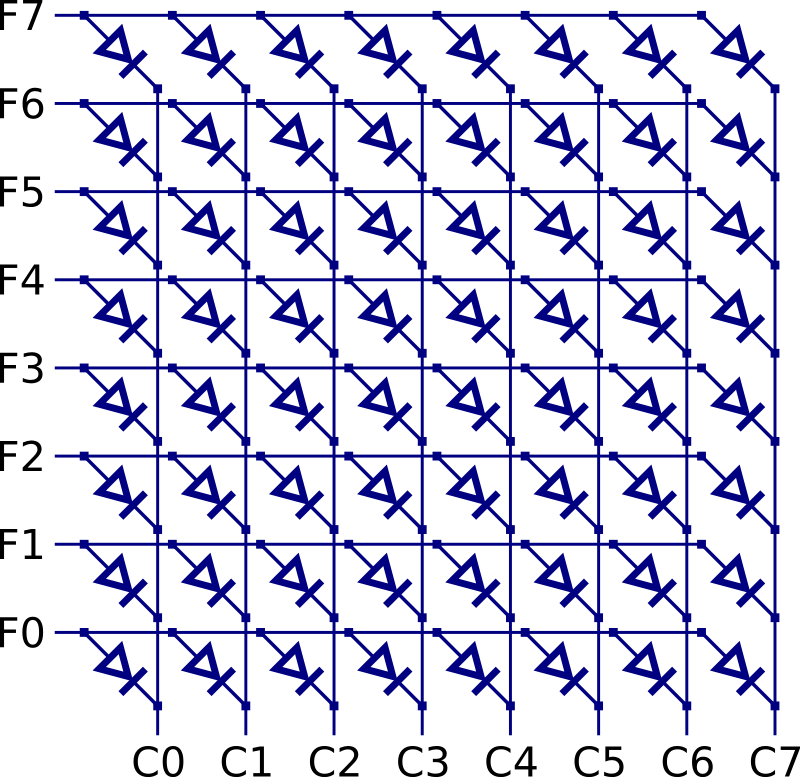
\includegraphics[width=200pt]{./images/esq_matriz.png}
\caption{Esquema de conexión de una matriz de LEDs 8x8.}
\label{fig:esq_matriz}
\end{figure}

La matriz puede fabricarse mediante la correcta colocación y conexionado de LEDs discretos, tal como ilustra la figura \ref{fig:esq_matriz}. Sin embargo, el número de contactos a conectar resulta lo bastante elevado como para resultar una labor tediosa: para una matriz de 8x8 se deben conectar 8x8x2=128 contactos. Existen en el mercado matrices ya empaquetadas con sólo el número de contactos correspondiente al número de filas y el número de columnas. Para una matriz de 8x8 se tendrían 8+8=16 contactos. La comodidad y el ahorro tanto en complejidad como en tiempo sin duda obligan a valorar muy positivamente esta posibilidad.

Para el desarrollo del prototipo de este proyecto, se ha utilizado un modelo comercial de 8x8\cite{matrix} del tipo columna-ánodo/fila-cátodo, debido a que era el modelo más accesible. Sin embargo, dado que la lógica se había considerado para una arquitectura donde las filas estuvieran conectadas a los ánodos, se ha optado por conectar los contactos descritos en la hoja de características como de columna a las filas, y viceversa.

La solución más rápida para gestionar una matriz de 8x8 mediante el microcontrolador consistiría en conectar cada uno de los contactos de ésta a un contacto del microcontrolador. Esto no resulta un problema para una matriz del tamaño descrito, pues disponemos de más 16 de contactos en el microcontrolador. Sin embargo, el objetivo de este proyecto es poder escalar el número de columnas para poder controlar carteles del tamaño deseado. Si se quisieran controlar 30 columnas, serían necesarios 38 contactos, de los cuales no se dispone. Es por esta razón por la que se ha optado por controlar la matriz de forma dinámica, haciendo uso de la multiplexación de las filas y utilizando registros de desplazamiento\cite{shiftr}.

Aprovechando que el microcontrolador funciona a una velocidad mucho mayor que la que el ojo humano es capaz de apreciar, se activarán las filas una por una, en lugar de encender todas ellas al mismo tiempo. Suponiendo que se trabaja con ocho filas, cada una de ellas estará encendida 1/8 parte del ciclo total de actualización. Como el ciclo total será menor que el tiempo mínimo apreciable, la sensación será la de estar viendo todas las filas iluminadas al mismo tiempo. Asumiendo que cada fila se encenderá por separado y nunca habrá dos de ellas activas al mismo tiempo, los LEDs que se encenderán vendrán determinados por el valor que tengan los contactos de las columnas en el momento de activación de una fila concreta. Ahí es donde cumplen su función los registros de desplazamiento: almacenarán los datos de las columnas durante el tiempo en que ésta esté activa. La comunicación entre el microcontrolador y un registro de desplazamiento es serie síncrona. Como es unidireccional, sólo necesitamos dos contactos, el de dato y el de reloj (que serán controlados por el microcontrolador), además de la masa.

De entre los registros de desplazamiento disponibles en el mercado, se ha optado por el 74HC164 \cite{164} en empaquetado PDIP de 14 contactos. Se trata de un modelo con dos contactos de entrada serie (1:A y 2:B), a las cuales se les realiza una operación lógica AND, y salida en paralelo de ocho bits. Puesto que no se necesitan las dos líneas de datos, se han conectado ambas entradas entre sí y al contacto de salida que se ha escogido en el microcontrolador para esta función (15:PB1). Las ocho salidas se han conectado a las respectivas columnas por medio de sendas resistencias \footnote{La función de las resistencias es limitar la tensión que caerá en los LEDs. El valor de éstas dependerá de la fuente con que se alimenten, como se verá al analizar la conexión de las filas.}, tal como describe la tabla \ref{tab:reg_col}.

\begin{table}[!htp]
\centering
\begin{tabular}[c]{|c|c|c|}
\hline
\multicolumn{2}{|c|}{\textbf{47HC164}} & \textbf{Matriz} \\
\hline
Q0 & 3 & C0 \\ \hline
Q1 & 4 & C1 \\ \hline
Q2 & 5 & C2 \\ \hline
Q3 & 6 & C3 \\ \hline
Q4 & 10 & C4 \\ \hline
Q5 & 11 & C5 \\ \hline
Q6 & 12 & C6 \\ \hline
Q7 & 13 & C7 \\
\hline
\end{tabular}
\caption{Conexiones entre el registro de desplazamiento y la matriz de LEDs.}
\label{tab:reg_col}
\end{table}

Los contactos de alimentación (14:VCC y 7:GND) se han conectado directamente a la fuente de alimentación. El reset global (9:$\overline{MR}$) se ha deshabilitado permanentemente dejándolo conectado a Vcc (el borrado se realizará por software al ejecutar la rutina de inicialización). El último contacto disponible, el de la señal de reloj (8:CP) se ha conectado al contacto escogido en el microcontrolador para dicha función (16:PB2).

Las salidas del microcontrolador pueden dar corriente suficiente para alimentar un reducido número de LEDs. Sin embargo, resulta claramente insuficiente a lo hora de trabajar con carteles de treinta, cuarenta o cincuenta columnas. En estos casos se debe utilizar un driver intermedio que actúe como etapa de potencia. Aunque el cartel del prototipo tiene pocas columnas, y a pesar de que en esas condiciones el microcontrolador podría alimentar los LEDs directamente, siempre es recomendable poner un driver para proteger el integrado de posible errores de montaje.

\begin{table}[!htp]
\centering
\begin{tabular}[c]{|c|c|c|}
\hline
\multicolumn{2}{|c|}{\textbf{Atmega48}} & \textbf{Matriz} \\
\hline
PC0 & 23 & F0 \\ \hline
PC1 & 24 & F1 \\ \hline
PC2 & 25 & F2 \\ \hline
PC3 & 26 & F3 \\ \hline
PC4 & 27 & F4 \\ \hline
PC5 & 28 & F5 \\ \hline
PD2 & 4  & F6 \\ \hline
PD3 & 5  & F7 \\
\hline
\end{tabular}
\caption{Conexiones entre el microcontrolador y la matriz de LEDs.}
\label{tab:filas}
\end{table}

En este proyecto las salidas del microcontrolador que deberán llevar driver son aquellas conectadas a las filas de la matriz de LEDs. Para conseguir la ganancia de potencia, se han utilizado transistores bipolares PNP\cite{140} que soportan una corriente de emisor de hasta 1.5A, lo cual permite conectar entre 75 y 100 columnas (en función de la corriente que consuman los LEDs). Al ser de tipo PNP, los transistores conducirán cuando la tensión en su base sea cero. Se debe tener en cuenta este hecho a la hora de realizar la programación de las rutinas del microcontrolador. Para desactivar una fila, por lo tanto, debería haber una tensión positiva en la base, lo cual se conseguirá activando la salida adecuada. Como sólo hace falta una pequeña corriente, se ha puesto una resistencia de 1K5 entre la salida y la base. El emisor de todos los transistores está conectado a la tensión de alimentación, mientras los colectores se conectan a las filas correspondientes de la matriz, de acuerdo con lo establecido por la tabla \ref{tab:filas}.

\begin{figure}[!htp]
\centering
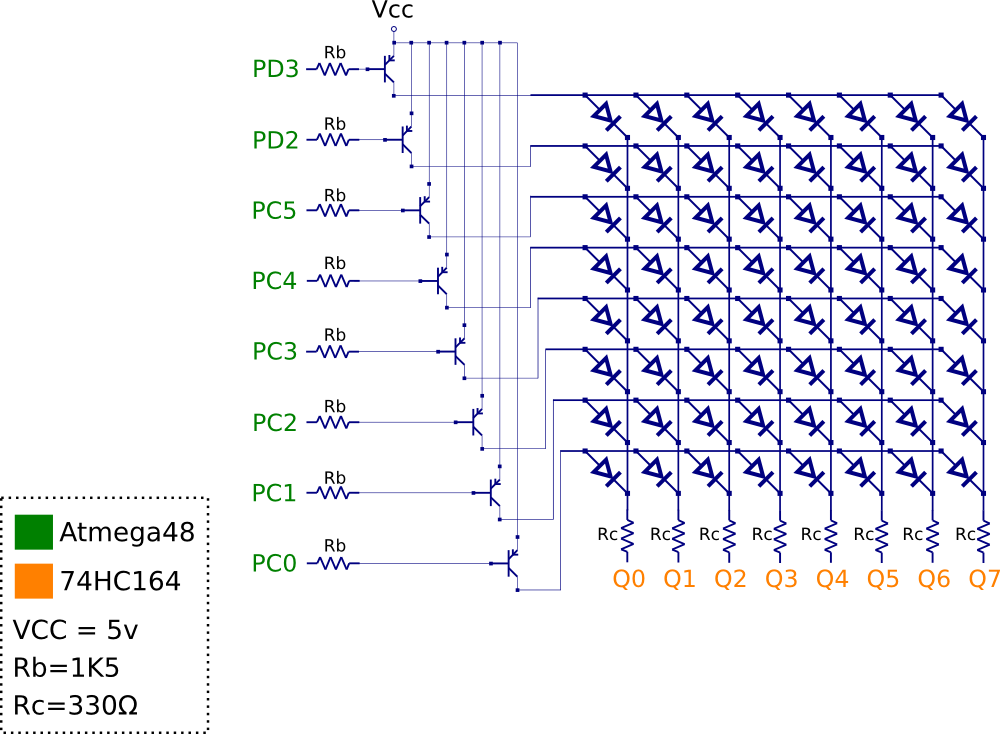
\includegraphics[width=350pt]{./images/esq_pnp.png}
\caption[Esquema de conexión matriz, microcontrolador y registro]{Esquema de conexión de la matriz al microcontrolador y al registro de desplazamiento.}
\label{fig:esq_pnp}
\end{figure}

Con la arquitectura descrita, cuando un transistor determinado conduzca y al menos una de las salidas del registro de desplazamiento esté a nivel bajo, habrá un LED que encuentre cero voltios (masa) en su cátodo y la tensión de alimentación en su ánodo. Lo más probable es que en estas condiciones el LED se queme, pues la alimentación será de aproximadamente cinco voltios. Para evitar que esto suceda, se podría sustituir la tensión en los emisores por una menor. Esto requiere dimensionar un divisor/reductor de tensión para soportar la corriente de todos los transistores. Desde un punto de vista práctico, resulta más fácil mantener ese mismo valor da alimentación e introducir resistencias entre los cátodos y las salidas del registro de desplazamiento, tal como ilustra la figura \ref{fig:esq_pnp}. Para el prototipo se han utilizado resistencias de 330$\Omega$.

\subsection{Programación}
\label{subsec:programacion}

Al ser el juego de instrucciones de la familia AVR desconocido para el desarrollador y no haber tenido nunca contacto con este tipo de microcontroladores, decidió para un primer acercamiento programar utilizando el lenguaje C, más concretamente el estándar ANSI. La arquitectura AVR está soportada por el compilador libre GCC\cite{gcc} y existe una implementación, también software libre, que permite utilizarlo bajo sistemas Windows, distribuida como WinAVR\cite{winavr} y que incluye compilador, programador y debugger.

Pese a la existencia de herramientas libres y multiplataforma para efectuar el desarrollo completo, se ha utilizado el AVR Studio 4\cite{avrstudio} como IDE. La elección de esta herramienta se justifica sólo por la seguridad de saber que se están utilizando recursos del propio fabricante que garantizan una alta compatibilidad con el kit de desarrollo. En cualquier caso, el uso de las herramientas de depurado y programación se escapan al objetivo de este documento, por lo que no se profundizará en su uso.

\subsubsection{Notas del desarrollador}

Si bien no son necesarias para la utilización del sistema, el desarrollador considera que las siguientes anotaciones pueden resultar de interés para quién quiera entender el desarrollo completo y qué decisiones se han tomado durante el mismo.

\begin{itemize}
  \item{\textbf{Estructura de ficheros}: la programación del microcontrolador se ha dividido en tres ficheros\footnote{El diagrama de flujo del programa completo se encuentra en el \hyperref[anexoc]{Anexo C}}:
    \begin{itemize}
      \item{\textbf{acher\_main.c}: contiene la función \textit{main} y las rutinas de vectorización de las interrupciones.}
      \item{\textbf{acher\_config.c}: contiene las rutinas de inicialización de variables y configuración de puertos y periféricos.}
      \item{\textbf{acher\_main.h}: contiene la declaración de constantes, variables y prototipos de las funciones.}
    \end{itemize}}
  \item{\textbf{Mayúsculas y minúsculas}: respetando la convención de código escrito en C, se han declarado los nombres de todas las constantes en mayúsculas, mientras las variables globales y las funciones aparecen en minúsculas. Todas ellas se encuentran declaradas en el fichero 'acher\_main.h'.}
  \item{\textbf{Estructura operativa de memorias}: se han utilizado tres matrices (arrays unidimensionales de tipo char/uint\_8t) que actúan implícitamente como memorias:
    \begin{itemize}
      \item{\textbf{leds[ ]}: su tamaño es proporcional al número de columnas declaradas. Actúa como buffer y contiene la información a mostrar bit a bit.}
      \item{\textbf{char\_ram[ ]}: su tamaño es proporcional al límite de caracteres definido. Actúa como RAM al almacenar los caracteres recibidos a través del puerto de serie. Los caracteres almacenados en esta memoria son los que irán volcándose a leds[] en un orden establecido.}
      \item{\textbf{CHAR\_ROM[ ]}: su tamaño es fijo. Contiene la equivalencia bit a bit en grupos de 8x5 píxeles para cada carácter del estándar ASCII. En otras palabras, define la tipografía para cada uno de los caracteres.}
    \end{itemize}}
  \item{\textbf{Operaciones con bits}: debido a que el compilador utilizado no permite la declaración de datos de tipo bit y como el microcontrolador no dispone de direccionamiento del mismo tipo, la modificación de bits determinados de un registro se ha realizado mediante máscaras implícitas. Así, se ha utilizado la operación lógica OR para poner a uno y la operación lógica AND para poner a cero. A continuación se muestra un ejemplo:

\begin{center}
\begin{tabular}[c]{ c | c }
Instrucción & Contenido de REG tras la ejecución \\ \hline
REG=0;			& 00000000 \\
REG$|$=(1$<<$3);	& 00001000 \\
REG\&=\~{}(1$<<$3);   	& 00000000 \\
\end{tabular}
\end{center}

\textit{1$<<$3} genera una máscara equivalente a desplazar un uno tres posiciones a la izquierda, es decir, \textit{00001000}. El operador \~{} complementa el contenido, luego, se obtiene \textit{11110111}. Las expresiones utilizadas son equivalentes a los valores binarios ahora descritos, o a sus equivalentes en cualquier otra base, por ejemplo, hexadecimal: 0x08 y 0xF7.

Más aún, la función \textit{\_BV(x)} actúa como \textit{1$<<$x}, generando una máscara con un uno desplazado \textit{x} posiciones a la izquierda y el resto ceros. Por lo tanto, \textit{\_BV(5)} == \textit{1$<<$5} == \textit{0b00100000}.
}
  \item{\textbf{$<$avr/io.h$>$}: al cargar la librería \textit{io.h} el compilador reconoce no sólo los nombres de los registros de función especial del microcontrolador, sino los nombres de los bits que éstos contienen. Aunque no está permitida la modificación de los bits directamente, sí pueden usarse sus nombres junto con las operaciones descritas en el apartado anterior. Así, para activar los bits RXEN0 y RXCIE del registro UCSR0B, se puede ejecutar la siguiente instrucción:

\begin{center}
UCSR0B$|$=(1$<<$RXEN0)$|$(1$<<$RXCIE0);
\end{center}

Equivalente a:

\begin{center}
UCSR0B$|$=(1$<<$RXEN0);

UCSR0B$|$=(1$<<$RXCIE0);
\end{center}

Se trata de una práctica que se ha reproducido a lo largo de todo el programa no sólo porque permite ver más claramente qué se está haciendo, sino también porque facilita la detección de errores (es más difícil confundirse en un nombre que en un número) y vuelve el código ligeramente más portable (algunos bits cambian de posición dentro del mismo registro entre los diferentes modelos de la familia AVR).
}
\end{itemize}

\subsubsection{acher\_main.c}

\begin{itemize}
\item{\textbf{Librerías y cabeceras}:
  \lstinputlisting[lastline=9]{acher_main.c}

  En primer lugar se han cargado las librerías necesarias para reconocer funciones y variables específicas.
  \begin{itemize}
    \item{\textbf{io.h}: reconoce el modelo de microcontrolador y permite utilizar nombres de registros específicos.}
    \item{\textbf{interrupt.h}: reconoce el sistema de interrupciones, declara funciones y vectores de interrupción específicos.}
    \item{\textbf{pgmspace.h}: declara funciones para permitir la declaración de constantes y variables en zonas de memoria concretas.}
    \item{\textbf{ina90.h}: declara las funciones específicas, entre ellas \_SLEEP() para entrar en modos de bajo consumo.}
    \item{\textbf{delay.h}: declara funciones para generar retardos mediante ticks.}
    \item{\textbf{acher\_main.h}: declara todas las variables y prototipos de funciones a utilizar.}
    \item{\textbf{acher\_config.c}: se definen las funciones y rutinas de inicialización y configuración.}
  \end{itemize}
}

\item{\textbf{Cuerpo del programa}:
  \lstinputlisting[firstnumber=last,firstline=10,lastline=19]{acher_main.c}

  La ejecución del programa sólo llama la rutina de configuración, \textit{config()} y entra continuamente en modo de bajo consumo. Sólo ``despierta'' para atender a las interrupciones. Después, vuelve a ``dormir''.
}

\item{\textbf{Rutina de tratamiento de la interrupción por recepción de la USART}:
  \lstinputlisting[firstnumber=last,firstline=20,lastline=25]{acher_main.c}

  Comprueba si hay espacio libre, si lo hay guarda el dato. Si el dato es una orden de borrado, reinicia el índice y desactiva las interrupciones de los temporizadores. Paso a Paso:
  \begin{itemize}
     \item{Si el índice de próximo carácter a escribir (\textit{show\_lim}) es menor que el máximo reservado (\textit{CHAR\_NUM}), es decir, si hay sitio libre en \textit{char\_ram}, guarda el dato recibido en el registro al que apunta \textit{show\_lim} dentro de \textit{char\_ram} e incrementa el índice.}
     \item{Si el dato recibido es el declarado como \textit{BORRAR}, se reinicia el índice.}
     \item{Mientras el índice sea cero, cuando la ram esté vacía, se desactivan las interrupciones de los Timers.}
  \end{itemize}
}

\item{\textbf{Rutina de tratamiento de la interrupción por comparación del Timer0}:
  \lstinputlisting[firstnumber=last,firstline=26,lastline=40]{acher_main.c}

  Carga el contenido a mostrar para cada fila y mantiene activa la fila hasta la siguiente interrupción. Paso a paso:
  \begin{itemize}
    \item{Desactiva todas las filas.}
    \item{Si el índice es igual a la última fila, se reinicia. Si no, se incrementa.}
    \item{Carga en la máscara \textit{line\_shadow} el índice de la fila a mostrar.}
    \item{Envía al registro de desplazamiento el bit indicado por la máscara de cada columna almacenada en el buffer (\textit{leds[ ]}).}
    \item{Activa la fila.}
  \end{itemize}
}

\item{\textbf{Rutina de tratamiento de la interrupción por comparación del Timer1}:
  \lstinputlisting[firstnumber=last,firstline=41,lastline=55]{acher_main.c}

  Modifica el contenido del buffer de acuerdo con la información presente en \textit{char\_ram}. Paso a paso:
  \begin{itemize}
    \item{Desplaza todas las columnas almacenadas en el buffer (\textit{leds[ ]}) una posición a la izquierda.}
    \item{Si el índice de columna se sale de rango (es uno más que la última columna del carácter) se escribe null en la última columna del buffer, se reinicia el índice, y se incrementa el índice de carácter. Además, si el índice de carácter se sale de rango (apunta al primer carácter vacío de la ram) se reinicia.}
    \item{Si no hay problemas de rango, escribe la columna de \textit{CHAR\_ROM} a la que apunta \textit{show\_col} dentro del carácter al que apunta \textit{show\_char} dentro de \textit{char\_ram}.}
  \end{itemize}
}

\item{\textbf{Rutina de envío de dato al registro de desplazamiento}:
  \lstinputlisting[firstnumber=last,firstline=56,lastline=68]{acher_main.c}

  Envía el bit recibido al registro de desplazamiento activando convenientemente la señal de reloj. Paso a paso:
  \begin{itemize}
     \item{Desactiva la señal de reloj.}
     \item{Si el dato recibido es diferente de cero, carga un cero en la línea de dato. Si es cero, carga un uno\footnote{Por el diseño realizado en el apartado \ref{subsubsec:muestra}, para activar un LED de la matriz la salida correspondiente del registro de desplazamiento debe estar a nivel bajo. Por lo tanto, en lo que al registro respecta, estamos trabajando con lógica negativa. De ahí que invirtamos el significado del dato recibido.}.}
     \item{Desactiva las interrupciones.}
     \item{Espera 1$\mu$s\footnote{De no hacerlo, no podríamos garantizar el correcto funcionamiento del registro de desplazamiento, pues en la hoja de características\cite{164} se especifica el tiempo mínimo que debe durar una transición en la línea de reloj.}.}
     \item{Activa la señal de reloj, cargando el dato en el registro de desplazamiento.}
     \item{Espera 1$\mu$s.}
     \item{Activa las interrupciones.}
   \end{itemize}
}

\item{\textbf{Función de escritura en los contactos conectados a las filas de la matriz}:
  \lstinputlisting[firstnumber=last,firstline=69]{acher_main.c}

  Escribe el valor correspondiente a cada contacto en los puertos y bits adecuados en función de las conexiones realizadas.
}
\end{itemize}

\subsubsection{acher\_config.c}

\begin{itemize}
\item{\textbf{Rutina de configuración e inicialización}:
  \lstinputlisting[lastline=13]{acher_config.c}

Llama a todas las subrutinas de configuración e inicialización, configura el modo de bajo consumo y activa las interrupciones. Se desactivan ADC, Timer2 y TWI durante el tiempo en que esté ``dormido''.
}

\item{\textbf{Configuración de los puertos}:
  \lstinputlisting[firstnumber=last,firstline=14,lastline=22]{acher_config.c}

  \begin{itemize}
    \item{Bits \textit{SHIFT\_DATA} y \textit{SHIFT\_CLK} del puerto B como salida.}
    \item{Las salidas del puerto B desactivadas.}
    \item{Todo el puerto C como salida.}
    \item{Todo el puerto C activado\footnote{Como el diseño se ha realizado con transistores PNP, éstos conducen cuando la tensión en base es nula. Activamos las salidas para que los transistores estén en corte.}.}
    \item{Bits 2 y 3 del puerto D como salida.}
    \item{Las salidas del puerto D activadas.}
  \end{itemize}
}

\item{\textbf{Inicialización de las variables}:
  \lstinputlisting[firstnumber=last,firstline=23,lastline=34]{acher_config.c}

  \begin{itemize}
  \item{Borra los índices de columna, de carácter y de ram, además de la máscara de filas.}
  \item{Borra todo el buffer y carga unos en el registro de desplazamiento.}
  \item{Borra toda la ram.}
  \item{El índice de fila apunta a la última, para reiniciarse en la primera interrupción.}
  \end{itemize}
}

\item{\textbf{Configuración de los Timers}:
  \lstinputlisting[firstnumber=last,firstline=35,lastline=54]{acher_config.c}

  \begin{itemize}
    \item{Borra el contador de los Timers 0 y 1.}
    \item{Define los límites de comparación para el Timer 0 (\textit{LINE\_LIMIT}) y el Timer 1 (\textit{COLUMN\_LIMIT}).}
    \item{Configura el modo y el prescaler para los Timers 0 y 1 (CTC, $clk_{I/O}$/1024).}
    \item{Limpia todos los flags de los Timers 0 y 1 (compA, compB, OV).}
    \item{Llama a la función \textit{timer\_int()} para activar las interrupciones de los Timers 0 y 1.}
  \end{itemize}
}

\item{\textbf{Configuración de la USART}:
  \lstinputlisting[firstnumber=last,firstline=55,lastline=65]{acher_config.c}

   Carga el valor calculado para un velocidad de 19200 baudios y configura el periférico para trabajar en modo asíncrono normal con 1 bit start, 8 bits data, no paridad y 1 bit stop. Limpia los flags de recepción y transmisión y habilita la recepción y la interrupción asociada. Deshabilita la transmisión.
}

\item{\textbf{Des/activación de las interrupciones de los Timers 0 y 1}:
  \lstinputlisting[firstnumber=last,firstline=66]{acher_config.c}

  Si el dato recibido como argumento es cero, se desactivan las interrupciones de los Timers 0 y 1. Si es diferente de cero, se activan.
}
\end{itemize}

\subsubsection{acher\_main.h}

\begin{itemize}
\item{\textbf{Definición de constantes}:
  \lstinputlisting[lastline=18]{acher_main.h}

  Se definen:
  \begin{itemize}
    \item{LINES: número de líneas de la matriz.}
    \item{COLUMNS: número de columnas de la matriz.}
    \item{CHAR\_NUM: capacidad de la ram.}
    \item{CHAR\_WIDTH: anchura de cada carácter (en columnas).}
    \item{BORRAR: código de borrado para la USART.}
    \item{SHIFT: puerto al que está conectado el registro de desplazamiento.}
    \item{SHIFT\_DATA: bit del puerto \textit{SHIFT} al que está conectado la entrada de dato del registro de desplazamiento.}
    \item{SHIFT\_CLK: bit del puerto\textit{SHIFT} al que está conectado la entrada de reloj del registro de desplazamiento.}
    \item{FREC: frecuencia de la señal de reloj, a utilizar para calcular el valor para la velocidad de transmisión y para las funciones de delay.}
    \item{BAUDRATE: velocidad de transmisión deseada (en baudios).}
    \item{UBR\_VAL: valor que debemos escribir en el registro de la USART para obtener una velocidad \textit{BAUDRATE} con una frecuencia \textit{FREC}.}
  \end{itemize}
}

\item{\textbf{Declaración de los prototipos de las funciones}:
  \lstinputlisting[firstnumber=last,firstline=19,lastline=28]{acher_main.h}

  Se declaran:
  \begin{itemize}
     \item{config(): rutina de inicialización y configuración.}
     \item{conf\_ports(): rutina de configuración e inicialización de puertos.}
     \item{conf\_variables(): rutina de inicialización de variables.}
     \item{conf\_timers(): rutina de configuración de los Timers 0 y 1.}
     \item{con\_serial(): rutina de configuración de la USART.}
     \item{shiftr\_write(): función para escribir un bit en el registro de desplazamiento.}
     \item{line\_write(): función para escribir en las salidas conectadas a las filas de la matriz.}
     \item{timer\_int(): función para des/activar las interrupciones de los Timers 0 y 1.}
  \end{itemize}
}

\item{\textbf{Declaración de variables}:
  \lstinputlisting[firstnumber=last,firstline=29,lastline=34]{acher_main.h}

  Se declaran:
  \begin{itemize}
    \item{show\_col: índice de columna dentro del carácter que se está cargando en el buffer.}
    \item{show\_char: índice de carácter dentro de la ram que se está cargando en el buffer.}
    \item{show\_lim: índice que apunta al próximo espacio libre en la ram.}
    \item{char\_ram[ ]: ram donde se almacenan los caracteres recibidos a través de la USART.}
    \item{leds[ ]: buffer donde se almacena el contenido que está mostrándose.}
    \item{line\_shadow: máscara para gestión de las filas.}
    \item{l: índice que apunta a la fila activa}
    \item{CHAR\_ROM[ ]: juego de caracteres almacenado en la zona de programa de la memoria del microcontrolador.}
  \end{itemize}
}

\end{itemize}

